
%(BEGIN_QUESTION)
% Copyright 2006, Tony R. Kuphaldt, released under the Creative Commons Attribution License (v 1.0)
% This means you may do almost anything with this work of mine, so long as you give me proper credit

Determine a basic 5-point (0\%, 25\%, 50\%, 75\%, and 100\%) calibration table for the displacer level transmitter in this scenario:

$$\includegraphics[width=15.5cm]{i00509x01.eps}$$

The cylindrical displacer weighs 9 pounds (dry) and has a diameter of 2 inches.  The process liquid is water.  The 0\% process liquid level (LRV) is even with the bottom of the displacer.  Assume an electronic transmitter mechanism with an output range of 4 to 20 mA.

% No blank lines allowed between lines of an \halign structure!
% I use comments (%) instead, so that TeX doesn't choke.

$$\vbox{\offinterlineskip
\halign{\strut
\vrule \quad\hfil # \ \hfil & 
\vrule \quad\hfil # \ \hfil & 
\vrule \quad\hfil # \ \hfil & 
\vrule \quad\hfil # \ \hfil \vrule \cr
\noalign{\hrule}
%
% First row
Process & Percent of & Buoyant & Output signal \cr
%
% Another row
level (in) & span (\%) & force (lb) & ideal (mA) \cr
%
\noalign{\hrule}
%
% Another row
  & 0 &  &  \cr
%
\noalign{\hrule}
%
% Another row
  & 25 &  &  \cr
%
\noalign{\hrule}
%
% Another row
  & 50 &  &  \cr
%
\noalign{\hrule}
%
% Another row
  & 75 &  &  \cr
%
\noalign{\hrule}
%
% Another row
  & 100 &  &  \cr
%
\noalign{\hrule}
} % End of \halign 
}$$ % End of \vbox

\underbar{file i00509}
%(END_QUESTION)





%(BEGIN_ANSWER)

% No blank lines allowed between lines of an \halign structure!
% I use comments (%) instead, so that TeX doesn't choke.

$$\vbox{\offinterlineskip
\halign{\strut
\vrule \quad\hfil # \ \hfil & 
\vrule \quad\hfil # \ \hfil & 
\vrule \quad\hfil # \ \hfil & 
\vrule \quad\hfil # \ \hfil \vrule \cr
\noalign{\hrule}
%
% First row
Process & Percent of & Buoyant & Output signal \cr
%
% Another row
level (in) & span (\%) & force (lb) & ideal (mA) \cr
%
\noalign{\hrule}
%
% Another row
{\bf 0} & 0 & {\bf 0} & {\bf 4} \cr
%
\noalign{\hrule}
%
% Another row
{\bf 5} & 25 & {\bf 0.567} & {\bf 8} \cr
%
\noalign{\hrule}
%
% Another row
{\bf 10} & 50 & {\bf 1.135} & {\bf 12} \cr
%
\noalign{\hrule}
%
% Another row
{\bf 15} & 75 & {\bf 1.702} & {\bf 16} \cr
%
\noalign{\hrule}
%
% Another row
{\bf 20} & 100 & {\bf 2.270} & {\bf 20} \cr
%
\noalign{\hrule}
} % End of \halign 
}$$ % End of \vbox

%(END_ANSWER)





%(BEGIN_NOTES)


%INDEX% Measurement, density: displacer (buoyancy)

%(END_NOTES)


